% Course report draft. Author and team confirmed by the user: Sheng Tao.
% Requires the unchanged aaai2026.sty and aaai2026.bst from the AAAI author kit.
% Open the official AAAI 2026 Overleaf template and copy these sources and figures.
\documentclass[letterpaper]{article}
\usepackage[draft]{aaai2026}
\usepackage{times}
\usepackage{helvet}
\usepackage{courier}
\usepackage[hyphens]{url}
\usepackage{graphicx}
\urlstyle{rm}
\def\UrlFont{\rm}
\usepackage{natbib}
\usepackage{caption}
\frenchspacing
\setlength{\pdfpagewidth}{8.5in}
\setlength{\pdfpageheight}{11in}
\pdfinfo{/TemplateVersion (2026.1)}
\setcounter{secnumdepth}{0}
\title{A Compact Residual Network for CIFAR-10 Under a Five-Million-Parameter Budget}
\author{Sheng Tao}
\affiliations{Deep Learning Course Project\\Kaggle Team: Sheng Tao}

\begin{document}
\maketitle

\begin{abstract}
We study CIFAR-10 classification under a limit of five million trainable
parameters, using only the images supplied by a course competition. A custom
residual network trained from random initialization achieves 96.64\% accuracy
on a fixed, stratified validation set of 5,000 images with 4,327,754 trainable
parameters. A smaller baseline achieves 94.04\%. Three completed experiments
compare a compact baseline, a wider network with Cutout, and an otherwise
identical wider network with Mixup. The final model correctly classifies 4,832
validation images and produces a checked prediction file for all 2,000 hidden
evaluation images. No pretrained weights, external training data, ensembles,
or test-time augmentation are used. These results are local validation results;
no Kaggle leaderboard score is available.
\end{abstract}

\section{Task and Data}
The course competition requires a custom convolutional network with residual
connections and at most 5,000,000 trainable parameters. Its local dataset
contains 50,000 labeled training images and 2,000 unlabeled evaluation images.
We validated every image as 32$\times$32 RGB and checked CSV columns, label
ranges, file existence, unique IDs, filenames, and submission ordering. Each
training class contains 5,000 images. There are no pixel-identical duplicates
within either supplied split.

Using seed 2026, we reserve 500 images per class for validation, leaving 45,000
training images and 5,000 validation images. The saved indices refer to rows in
the original training CSV, whose hash is recorded. There are no pixel-identical
images across the training/validation boundary. Channel normalization statistics
are calculated exclusively from the 45,000 training images. Hidden evaluation
images do not participate in optimization, normalization, or model selection.

\section{Architecture}
Residual connections permit a block to learn a residual transformation in
addition to a shortcut \citep{he2016resnet}. We implement post-activation blocks
of the form
\begin{equation}
 h = \operatorname{ReLU}\big(F(x)+S(x)\big),
\end{equation}
where $F$ contains two 3$\times$3 convolutions with batch normalization and an
intermediate ReLU. The shortcut $S$ is the identity when dimensions agree;
otherwise it is a 1$\times$1 convolution followed by batch normalization.

Our CIFAR-specific stem is a 3$\times$3 convolution with stride one. Three stages
each contain three residual blocks. The first block of stages two and three
uses stride two; the other blocks preserve resolution. Global average pooling
feeds a ten-class linear classifier. The baseline uses stage widths 32, 64,
and 128. The wider candidates use 64, 128, and 256, following the general
motivation of wider residual representations \citep{zagoruyko2016wide}; our
implementation is not an exact reproduction of the published WRN architecture.

The baseline has 1,084,586 trainable parameters. Both wider candidates have
4,327,754, including batch-normalization affine parameters, projection shortcuts,
and the classifier. The implementation counts and asserts the parameter limit
before training and prediction. Every candidate starts from random initialization.

\section{Training Protocol}
We use SGD with Nesterov momentum 0.9, weight decay $5\times10^{-4}$, batch size
128, and base learning rate 0.1. A linear warmup is followed by a per-step cosine
decay, using the cosine scheduling principle of \citet{loshchilov2017sgdr}
without warm restarts. The minimum learning-rate ratio is 0.001. The baseline
uses three warmup epochs and 60 total epochs; the wide models use five warmup
epochs and 160 total epochs. Label smoothing is disabled.

All models receive independent random 32$\times$32 crops after four-pixel
reflection padding and random horizontal flips. Wide models additionally use
Cutout with a 16$\times$16 mask, clipped at image boundaries
\citep{devries2017cutout}. The final candidate also uses Mixup with
$\alpha=0.2$ \citep{zhang2018mixup}. For a random pair of training examples,
we sample $\lambda\sim\operatorname{Beta}(\alpha,\alpha)$ and optimize the
weighted cross-entropy of their mixed inputs and two original targets.
Validation uses unaugmented images and ordinary cross-entropy.

Experiments run sequentially on a Windows NVIDIA RTX 4060 Laptop GPU with
8 GB dedicated memory, using Python 3.11.4, PyTorch 2.6.0 with CUDA 12.4,
BF16 autocast, and channels-last tensors. The compact dataset is cached as
unsigned-byte tensors on the GPU. A three-epoch pilot verifies forward/backward
execution and recovery from a saved one-epoch checkpoint. All formal runs save
per-epoch metrics and both latest and best checkpoints. Selection uses the
highest validation accuracy, breaking ties by lower validation loss.

\section{Results}
Table~\ref{tab:results} reports completed experiments. Timings sum the recorded
training epoch process, excluding environment installation, initial data auditing,
and separate inference. Total formal training time is 3,874.03 seconds
(64.57 minutes). Figure~\ref{fig:curves} shows the validation trajectories.

\begin{table*}[t]
\centering
\begin{tabular}{lrrrrrr}
\hline
Configuration & Parameters & Epochs & Best epoch & Logged best & Re-evaluated & Seconds \\
\hline
Baseline & 1,084,586 & 60 & 59 & 94.04\% & 94.04\% & 249.77 \\
Wide + Cutout & 4,327,754 & 160 & 158 & 96.32\% & 96.30\% & 1,812.07 \\
Wide + Cutout + Mixup & 4,327,754 & 160 & 158 & 96.64\% & 96.64\% & 1,812.19 \\
\hline
\end{tabular}
\caption{Actual results on the same fixed validation split. Logged best is measured
during training; re-evaluated accuracy is measured after separately loading the
selected checkpoint. The Cutout discrepancy is one image under BF16/cuDNN numerical
variation. Baseline-to-Wide comparisons change multiple factors.}
\label{tab:results}
\end{table*}

\begin{figure*}[t]
\centering
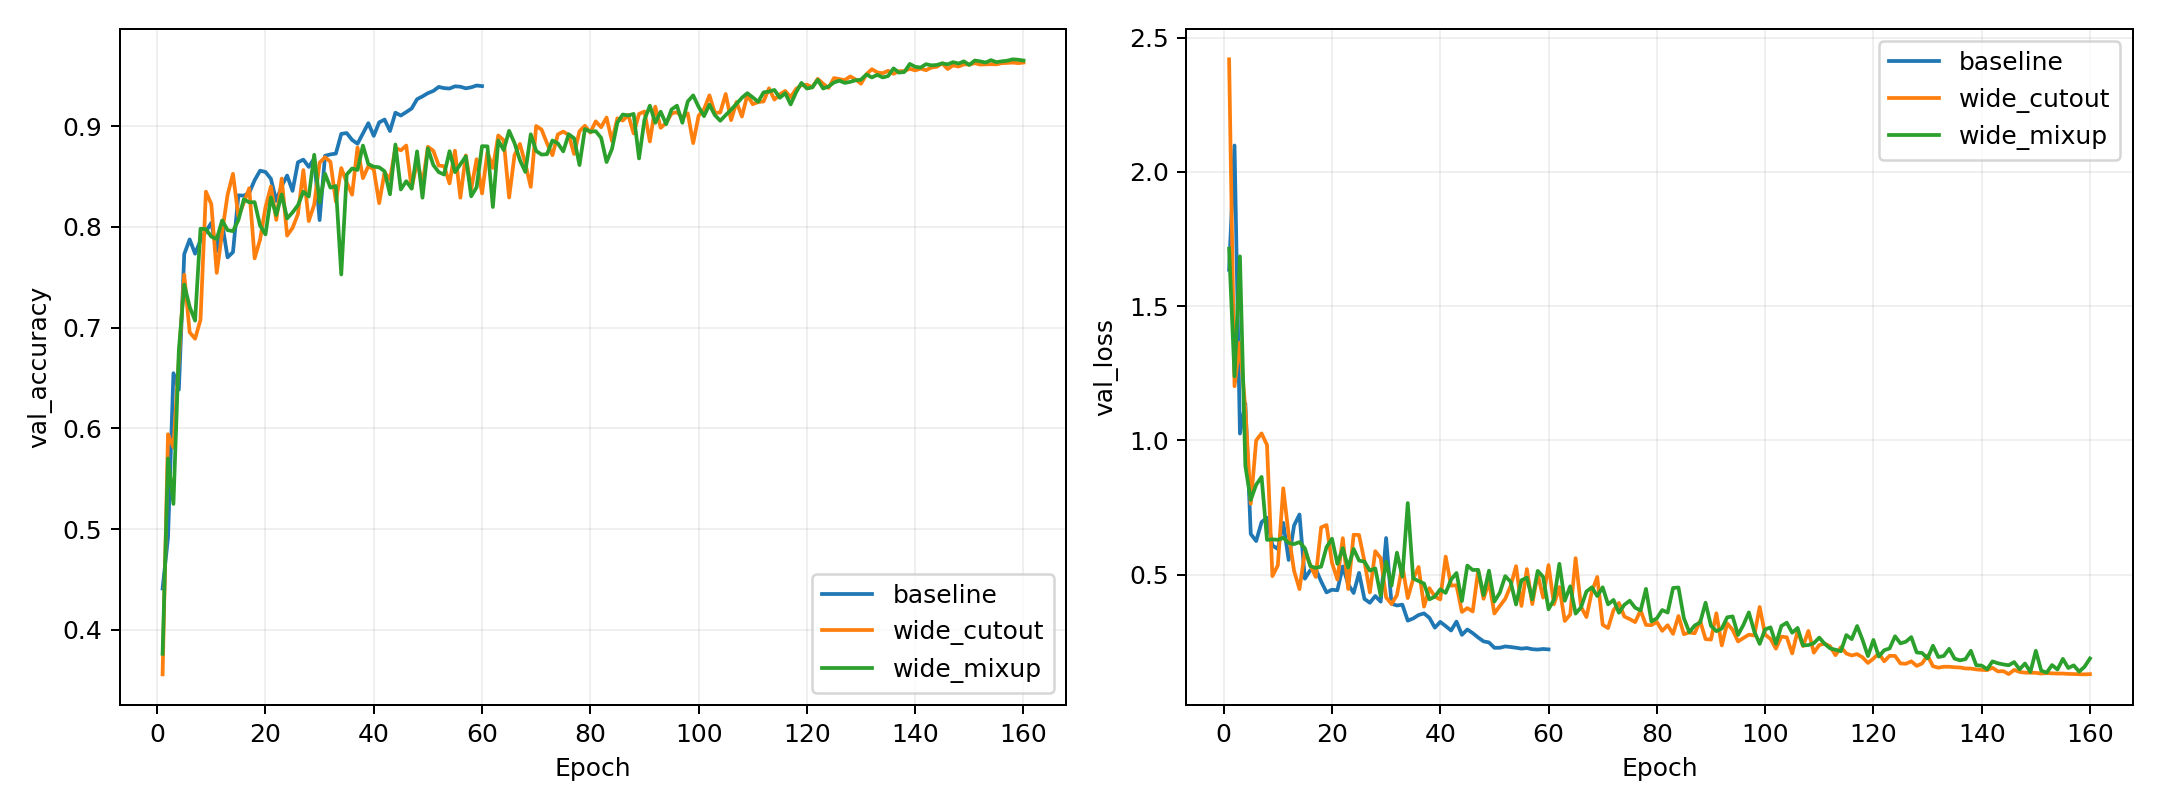
\includegraphics[width=\textwidth]{figures/training_curves.png}
\caption{Validation accuracy and loss from the saved epoch logs. Wider models use
a longer schedule than the baseline; this comparison does not isolate architecture
from training duration and regularization.}
\label{fig:curves}
\end{figure*}

The selected Mixup model obtains 96.64\% accuracy (4,832/5,000) and validation
cross-entropy 0.13903644. It improves over the baseline by 2.60 percentage points,
or 130 correct predictions. The two wide experiments differ only in whether
Mixup is enabled. In independent re-evaluation, Mixup improves accuracy by 0.34
percentage points, or 17 images: 81 images are correct only for the Mixup model,
while 64 are correct only for the Cutout model. Cutout alone has lower validation
cross-entropy (0.12930883), so the choice of Mixup follows the competition's
accuracy metric rather than minimum loss.

Two independent evaluations of the final checkpoint yield the same 96.64\%
accuracy. Two separately generated prediction files are byte-identical. The
descriptive Wilson 95\% interval for its validation accuracy is approximately
96.10--97.10\%; this interval does not correct for selecting configurations and
epochs using the same validation set.

Class-level evaluation shows the lowest accuracy for class ID 3 (91.6\%) and
class ID 5 (94.0\%). Confusions between these two IDs account for 44 validation
errors. The full confusion matrix and per-class scores are retained with the
experiment artifacts. Numeric class IDs are used without assuming an externally
derived label mapping.

\section{Prediction and Reproducibility}
The final checkpoint is epoch 158 of the 160-epoch Mixup run. We retain the
45,000-image training model to preserve a directly re-evaluable checkpoint,
rather than retraining on all 50,000 images. Prediction uses one model in
evaluation mode with inference-mode autograd disabled, without test-time
augmentation or ensembling.

The submission writer maps each image through the explicit test CSV ID and
filename relationship, then preserves the official sample-submission ID order.
The resulting file has exactly two columns, \texttt{id,label}, and 2,000 rows;
IDs are unique and labels are integers in 0--9. Checkpoint and prediction hashes,
data-audit results, split indices, complete configurations, source snapshots,
training logs, and environment versions are saved. A resumption checkpoint
includes the optimizer and random generator states. CUDA bitwise determinism
across hardware or library versions is not claimed.

\section{Limitations and Course Handoff}
Only one fixed split and one seed were used. Repeated epoch/configuration
selection may make the reported validation result optimistic. The relatively
small Mixup gain needs repeated-seed evidence before being generalized. The
baseline comparison simultaneously changes width, regularization, warmup, and
training length, so their individual contributions cannot be separated. No
hidden-test accuracy or leaderboard ranking is asserted.

The sole team member is Sheng Tao, and the Kaggle team name is Sheng Tao.
The private GitHub repository is available at
\url{https://github.com/TolsonRyan/cifar10-resnet-architecture-challenge}.
Course registration and final
formatting requirements must be confirmed by the team. The prediction file
has not been submitted to Kaggle. This report
is a student-editable draft; implementation and documentation assistance are
disclosed separately in \texttt{TOOL\_USAGE.md}.

\bibliographystyle{aaai2026}
\bibliography{references}
\end{document}
